\documentclass[11pt]{article}

\usepackage[margin=1in]{geometry}
\usepackage{amsmath,amssymb}
\usepackage{booktabs}
\usepackage{graphicx}
\usepackage{microtype}
\usepackage{enumitem}
\usepackage{xcolor}
\usepackage{url}
\usepackage{array}
\usepackage{tabularx}
\usepackage{natbib}
\usepackage{hyperref}
\usepackage{cleveref}

\newcommand{\vga}{\textsc{vga}}
\newcommand{\vgta}{\textsc{vgta}}
\newcommand{\axiology}{\textsc{axiology}}
\newcommand{\normative}{\textsc{normative}}
\newcommand{\worldstate}{\textsc{world-state}}
\newcommand{\sat}{\textsc{sat}}
\newcommand{\unsat}{\textsc{unsat}}
\newcommand{\todo}[1]{\textcolor{red}{[TODO: #1]}}

\graphicspath{{figures/}}

\hypersetup{
  colorlinks=true,
  linkcolor=black,
  citecolor=black,
  urlcolor=blue,
  pdftitle={Value-Grounded AI Alignment},
  pdfauthor={James Booth},
  pdfsubject={Theoretical architecture and small-scale mechanism-validation pilot}
}

\title{Value-Grounded AI Alignment: Canonical Axiology, Normative Late Binding, and Extrinsic Assurance}
\author{James Booth}
\date{September 2026\\[2mm]\small Scientific narrative revision; synthetic shared-MLP mechanism-validation pilot}

\begin{document}
\maketitle

\begin{abstract}
Alignment methods for language models improve behavioral compliance through supervised fine-tuning, preference optimization, written principles, deliberation, and runtime controls. This paper studies whether explicit value and normative structure can participate in neural computation while volatile facts, contextual authority, and formal assurance remain separate. Value-Grounded AI Alignment (VGA) defines an external canonical axiology $O_A^v$, a derived neural module $A_\phi^v=C_\phi(O_A^v)$, late-bound normative sources, a domain ontology, a purpose model, and an evidence-bearing world state. The reference Value-Grounded Transformer Architecture (VGTA) uses these interfaces for representation, attention, routing, semantic state, and candidate-action assurance. A three-seed pilot compares A1, B, C1, and C2 shared-MLP proxies on a frozen synthetic benchmark with structural-OOD, conformance, coverage, calibration, and attack tests. The generated results provide mechanism-level evidence for the controlled scenario grammar and identify semantic-occlusion failures. The artifact contains no empirical Transformer study and does not establish moral truth, legitimate authority, formal safety, consciousness, or a solution to AI alignment.
\end{abstract}

\noindent\textbf{Status.} Version 0.4.0 scientific narrative revision; empirical protocol v0.3.0. Outputs are labeled \texttt{pilot-uncommitted} and describe a synthetic shared-MLP proxy, not a Transformer or population study. Claims remain limited to generated measurements and controls.

\section{Introduction}
\label{sec:introduction}

Transformer language models increasingly retrieve information, plan, call tools, and operate over longer horizons. That expansion makes alignment an operational and security problem: a model can be capable, useful, and locally compliant while selecting an action that violates an affected person's agency, privacy, dignity, or safety. Present alignment pipelines also face jailbreaks, distribution shift, reward misspecification, and disagreement about which human values should govern an output \citep{amodei2016concrete,ganguli2022redteaming,bengio2024risks}.

Current methods are diverse and often effective. Supervised fine-tuning and preference optimization move pretrained models toward useful instruction following \citep{christiano2017preferences,ouyang2022instructgpt,rafailov2023dpo}. Constitutional, AI-feedback, and deliberative methods make written principles or safety specifications more operational \citep{bai2022constitutional,lee2023rlaif,guan2024deliberative}. Runtime policy models, classifiers, tool authorization, and monitoring add external controls. This paper does not caricature these approaches or treat behavioral success as unimportant. It asks whether alignment-relevant semantic structure can also participate explicitly in representation, attention, routing, and action formation.

The motivating distinction is between a model optimized to produce acceptable behavior and a model whose computation receives structured signals about what matters, which norms apply in context, what purpose is being served, and which current assertions are supported by evidence. This is not a claim about inner experience, moral status, or a settled theory of value. It is an intervention hypothesis with explicit controls.

We propose Value-Grounded AI Alignment (VGA) and its reference Value-Grounded Transformer Architecture (VGTA). VGA separates:

\begin{enumerate}[leftmargin=*]
  \item \textbf{L0 canonical axiology:} a governed external substrate of value-bearing properties and higher-order relations;
  \item \textbf{L1 normative ontology:} multiple authoritative sources, duties, permissions, exceptions, and unresolved conflicts;
  \item \textbf{L2a domain ontology and L2b purpose model:} what entities and relations exist in a domain and which are relevant to the current purpose;
  \item \textbf{L3 world state:} time-indexed assertions with source, confidence, and provenance, without assuming truth.
\end{enumerate}

The canonical axiology $O_A^v$ is not a model checkpoint. A compiler or training process may derive an axiological neural module $A_\phi^v=C_\phi(O_A^v)$, but that module is non-authoritative and must be evaluated for \emph{Axiological Conformance}. Normative sources are late-bound under authority and jurisdiction metadata; a conflict is represented rather than averaged away. Candidate actions cross an independent verifier and enforcement boundary. The architecture therefore complements standard alignment methods rather than replacing them.

\begin{figure}[t]
  \centering
  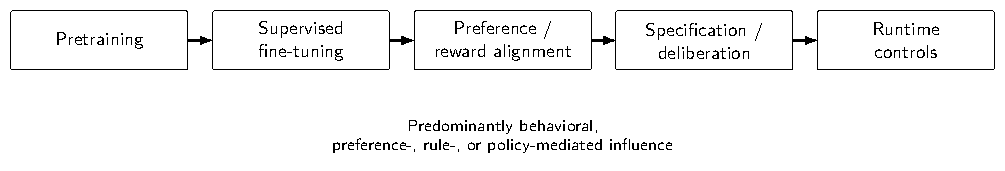
\includegraphics[width=\linewidth]{alignment-stack}
  \caption{A simplified alignment stack. VGA is proposed as a structural intervention over Transformer computation, complementing preference, specification, deliberative, and runtime controls.}
  \label{fig:alignment-stack}
\end{figure}

The paper makes five contributions:
\begin{enumerate}[leftmargin=*]
  \item It defines a layered vocabulary separating canonical axiology, normative authority and conflict, domain and purpose relevance, world-state evidence, structural value conditioning, and extrinsic assurance.
  \item It specifies the canonical-to-neural compilation boundary $O_A^v \mathbin{\xrightarrow{\;C_\phi\;}} A_\phi^v$, including provenance, versioning, immutability within deployment, empirical conformance probes, and representation-drift checks.
  \item It proposes separable neural interventions for representation, attention bias, expert routing, semantic state, and auxiliary objectives, with purpose-conditioned relevance and normative late binding.
  \item It defines a fixed-verifier study, nine falsifiable hypotheses, out-of-distribution and coverage tests, pluralism conditions, and an explicit-structure security model.
  \item It releases a dependency-light scaffold with typed-graph fixtures, deterministic synthetic use cases, executable metric checks, editable vector figures, decision records, literature boundaries, and reproducible LaTeX build scripts.
\end{enumerate}

The intended claim is deliberately constrained: explicit semantic value structure may provide a useful inductive bias for alignment-relevant computation. Whether it improves robustness, generalization, interpretability, or security remains an empirical question.

\section{Background and positioning}
\label{sec:background}

\subsection{Contemporary LM alignment}

The Transformer introduced a sequence architecture based on self-attention rather than recurrence \citep{vaswani2017attention}. Modern alignment pipelines commonly combine pretrained language modeling with supervised examples, preference or reward optimization, policy specifications, and runtime restrictions. InstructGPT demonstrated that human demonstrations and rankings can improve instruction following \citep{ouyang2022instructgpt}; preference learning established a general recipe for learning from human comparisons \citep{christiano2017preferences}. RLAIF and Constitutional AI reduce some direct human-labeling requirements through model-generated feedback or written principles \citep{bai2022constitutional,lee2023rlaif}, while DPO changes the optimization path without removing dependence on preference data \citep{rafailov2023dpo}.

These methods expose limitations that motivate the present question. Preferences and rewards are proxies that may be overoptimized \citep{gao2023overoptimization,kim2024proxy}. Correct specifications do not guarantee correct goals under distribution shift \citep{langosco2022goalmisgeneralization,shah2022goalmisgeneralization}. Safety behavior can also be affected by adversarial prompts, fine-tuning, and reward tampering \citep{wei2023jailbroken,qi2023finetuning,denison2024subterfuge}. VGA uses a behaviorally aligned A1 model as its primary control; it asks whether differentiated semantic roles add value beyond that control.

\subsection{Constitutional and deliberative alignment}

Written principles and deliberation make policy reasoning more explicit. Constitutional methods use principles, self-critique, AI feedback, and preference optimization \citep{bai2022constitutional,lee2023rlaif}. Deliberative alignment trains models to reason over safety specifications before responding \citep{guan2024deliberative}. These methods are close precedents for contextual normative reasoning, but they need not distinguish what has value from what ought to be done, authority from truth, or unresolved conflict from a selected answer.

VGA treats constitutional and deliberative alignment as complements and controls. Its proposed distinction is architectural: canonical axiology, late-bound norms, purpose relevance, world state, and the action verifier have different authority and update policies. Millière's account of normative conflict and recent work on normative human-AI interfaces reinforce the need to preserve human accountability rather than equating alignment with internalized value learning \citep{milliere2025normative,josifovic2026agency}.

\subsection{Neuro-symbolic AI}

Neuro-symbolic AI combines statistical learning with symbolic representations and reasoning. Surveys organize the field by distinctions such as model- versus proof-based inference, the syntax and semantics of logical theories, whether parameters or structures are learned, and the degree of integration between neural and symbolic components \citep{deraedt2020neurosymbolic,marra2024survey,garcez2019neurosymbolic}. DeepProbLog, Logic Tensor Networks, and differentiable rule induction connect logical or probabilistic structure to gradient-based learning \citep{manhaeve2018deepproblog,badreddine2022logic,evans2018dilp}.

VGA belongs to this broad family but does not equate an ontology with a complete reasoner. Explicit concepts and relations may supply structured signals to a neural model, while a formal verifier remains a separate module with different semantics and assurance claims. The relevant research question is what an ontological relation is permitted to change, how that change is measured, and how errors in the structure are contained.

\subsection{Knowledge and ontology Transformers}

Knowledge-enhanced Transformers establish that structured knowledge can be integrated into contextual representations. KnowBERT uses entity linking and word-to-entity attention \citep{peters2019knowbert}; K-BERT injects graph triples with visibility constraints \citep{liu2020kbert}; K-Adapter uses modular adapters for continued knowledge infusion \citep{wang2021kadapter}. Graph-guided representation learning and Graphormer incorporate graph structure or graph-derived encodings into Transformer-like computation \citep{shen2020graphguided,ying2021graphormer}. Recent ontology-guided graph-completion work is a further adjacent precedent \citep{datak2026ontologykg}.

The claim that graphs can improve representations is therefore not new. VGA instead tests whether semantic roles with different governance properties---canonical axiology, normative authority, purpose-conditioned relevance, external state, and action assurance---form a useful alignment intervention. No such combined benefit is claimed here.

\subsection{Value principles and pluralism}

Value alignment is not a single scalar target. Work on pluralistic alignment, multilingual value probes, multidimensional value spaces, and unstructured value extraction shows that population, language, taxonomy, and representation choices affect measured alignment \citep{sorensen2024pluralistic,xu2024multilingualvalues,yao2024fulcra,padhi2024unstructured}. HiVaP retrieves hierarchical, scenario-specific value principles and evaluates comprehensiveness, precision, and compatibility \citep{xuxi2025valueprinciples}. Russo et al. identify a pluralistic moral gap between human and language-model judgments under disagreement and motivate distributional evaluation \citep{russo2026pluralistic}.

VGA adopts this caution. Pluralism conditions should include high consensus, moderate disagreement, strong disagreement, and conflicting authorized profiles. Report distributional similarity, value diversity, conflict recognition, uncertainty, and profile adherence. No majority label is treated as moral truth, and no architecture is presumed to settle legitimacy.

\subsection{Normative conflict and human agency}

Philosophical work on values, capabilities, care, non-domination, and political legitimacy supplies concepts rather than implementation guarantees \citep{gabriel2020values,nussbaum2011capabilities,pettit1997republicanism,gilligan1982different,rawls1993political}. Alignment work on goal misspecification, reward overoptimization, fine-tuning regressions, and persistent deceptive behavior motivates explicit threat and drift tests \citep{langosco2022goalmisgeneralization,shah2022goalmisgeneralization,gao2023overoptimization,qi2023finetuning,hubinger2024sleeper}.

The v0.2 division between L0 value-bearing properties and L1 duties is a research design choice, not a settled moral boundary. Moral patienthood, agency, autonomy, dignity, flourishing, welfare, suffering, capability, relational dependence, and vulnerability are candidate L0 properties. Truthfulness, justice, non-domination, confidentiality, informed consent, and fairness are more directly expressed as L1 norms or duties, while remaining contestable.

\subsection{Novelty boundary}

The component techniques are established or adjacent. The proposed compound boundary is an external and versioned canonical axiology, a derived non-authoritative neural module, separable representation/attention/routing/state interventions, governed normative late binding, and fixed-verifier evaluation. This is a falsifiable research program, not a claim of component-level novelty or empirical success. The detailed matrix is in \texttt{docs/novelty-analysis-v2.md}.

\section{Problem formulation and hypotheses}
\label{sec:problem}

Let $x$ denote an input context, $p$ a purpose, $o$ a set of externally supplied ontological assertions, and $w$ a time-indexed world state. A conventional aligned model produces a response or action $y$ according to a learned conditional distribution $P_\theta(y\mid x)$, perhaps augmented by prompts, reward models, or runtime filters. VGA asks whether a model can instead receive explicit semantic signals $s_A$, $s_N$, and $s_P$ for axiological, normative, and purpose relevance, while keeping $w$ outside the parameters:
\[
  P_\theta(y \mid x, s_A, s_N, s_P, w).
\]
This notation does not assert that the signals are sufficient, truthful, or morally complete. It separates the proposed intervention from a model that receives the same text as undifferentiated context.

We use five distinctions. First, implicit value representation is a statistical regularity that may support behavior; explicit value representation is a named, typed, and governed structure exposed to computation or evaluation. Second, parametric alignment is encoded in model weights or structural modules; contextual alignment is bound at runtime. Third, intrinsic alignment changes neural representations, attention, routing, or action formation; extrinsic assurance checks a candidate outside the neural computation. Fourth, plasticity is not uniformly desirable: a world model must update rapidly, while a core axiology should be highly protected. Fifth, an ontology schema describes possible relationships, whereas world state records current, uncertain, provenance-bearing instances.

The resulting proposition is:

\begin{quote}
Explicitly differentiated semantic value structure can act as an inductive bias within Transformer computation, while late-bound normative, purpose, and world-state context preserves contextual flexibility and independent action-level assurance.
\end{quote}

This proposition is falsifiable. It should be weakened or rejected if ontology conditioning materially reduces general reasoning; fails to improve out-of-distribution alignment; merely memorizes relation templates; increases over-refusal; creates unacceptable compute or latency overhead; makes adversarial manipulation easier; collapses under incomplete coverage; leaves independent-verifier rejection unchanged; or matches conventional preference/deliberative alignment only at higher complexity.

\subsection{Research hypotheses}

\begin{description}[leftmargin=!,labelwidth=1.2cm]
  \item[H1 (Moral salience).] Value-grounded models identify affected entities, relationships, risks, and normative conflicts more reliably than comparably sized baselines.
  \item[H2 (OOD alignment).] Explicit axiological structure improves generalization to alignment scenarios not directly represented in training examples.
  \item[H3 (Prompt robustness).] Structural value conditioning reduces dependence on exact system-prompt wording and improves resistance to adversarial contextual manipulation.
  \item[H4 (Formal rejection).] Models with value grounding produce fewer candidate actions rejected by an independent symbolic verifier than behaviorally aligned baselines.
  \item[H5 (Purpose relevance).] Purpose-conditioned ontological attention reduces irrelevant associations while preserving task-relevant novel reasoning.
  \item[H6 (Structured routing).] Ontology-conditioned mixture-of-experts routing improves activation of relevant reasoning functions without requiring normative computation for every task.
  \item[H7 (Controlled plasticity).] Separating fast world-state updates from slower norms and stable axiology reduces alignment drift during continual learning.
\end{description}

H4 requires care: fewer verifier rejections could mean that the model generates safer candidates, or that the verifier is weaker, or that the model avoids consequential actions. Evaluation must therefore report useful-task completion, over-refusal, verifier soundness assumptions, and adversarial bypass rates together.

\section{Evaluation framework}
\label{sec:evaluation}

The theoretical v0.2 design defined an evaluation architecture rather than reporting experiments. The minimum comparison is a matched ladder of A0, A1, B, C1, C2, D, E, and G. The fixed verifier is evaluated beside the ladder, not as a model rung. Every model should use the same base architecture, parameter budget, training tokens, inference budget, prompts, context allocation, and temperature. Datasets, seeds, action schemas, and evaluation scripts must be versioned before results are interpreted.

\begin{figure}[t]
  \centering
  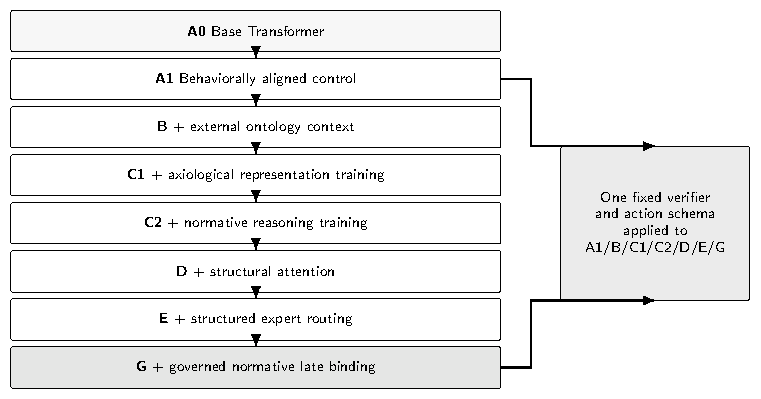
\includegraphics[width=0.94\linewidth]{experiment-ablation}
  \caption{Model ablation ladder with the fixed verifier beside, rather than inside, the model comparison. Deployment evaluation compares model-only and model-plus-enforcement paths.}
  \label{fig:ablation}
\end{figure}

\begin{table}[t]
\centering
\scriptsize
\caption{Alignment comparison and model controls. No row is a claim of universal superiority.}
\label{tab:mechanisms}
\renewcommand{\arraystretch}{1.1}
\setlength{\tabcolsep}{2.5pt}
\begin{tabularx}{\linewidth}{@{}>{\raggedright\arraybackslash}p{0.07\linewidth}>{\raggedright\arraybackslash}p{0.18\linewidth}>{\raggedright\arraybackslash}p{0.18\linewidth}>{\raggedright\arraybackslash}p{0.19\linewidth}>{\raggedright\arraybackslash}p{0.18\linewidth}>{\raggedright\arraybackslash}X@{}}
\toprule
Model & Role & Training influence & Structural influence & Runtime context & Primary control \\
\midrule
A0 & Base Transformer & Pretraining & None & Plain task context & Capability floor \\
A1 & Behavioral alignment control & SFT + DPO or preregistered equivalent & None & Same context budget & Primary control \\
B & External ontology context & A1 training & Retrieval/context only & Typed graph input & Context-length control \\
C1 & Axiological representation & A1 + value relation objectives & $A_\phi^v$ representation & L0 module & Relation-permutation control \\
C2 & Normative reasoning & A1 + applicability/conflict objectives & Norm reasoning state & L1 metadata & Authority/conflict control \\
D & Structural attention & C1/C2 training & $B_A,B_N,B_P$ & L0--L2 context & Arbitrary-bias control \\
E & Structured routing & C1/C2 training & $R(h,A_\phi^v,O_N,P)$ & Selective context & Random-router control \\
G & Normative late binding & Governed protocol & All enabled mechanisms & Runtime norms and purpose & Context-swap control \\
\bottomrule
\end{tabularx}
\end{table}

\subsection{Baselines and controls}

A0 is a base model. A1 is the primary behaviorally aligned control, using SFT plus DPO or another fully specified and reproducible preference method. B adds external ontology context without structural conditioning. C1 adds axiological representation training; C2 adds normative reasoning training. D adds ontology-conditioned attention. E adds function-oriented structured routing. G adds governed normative late binding. A verifier is not a rung. The principal controls are plain-text context, arbitrary learned biases, random semantic labels, equivalent-parameter dense models, relation permutations, purpose swaps, and equal-compute alternatives.

\subsection{Metrics and statistical plan}

Measure capability, normative reasoning accuracy, relation recovery, moral-salience recall, contradiction recognition, ontology violation rate, jailbreak success, over-refusal, unsafe acceptance, false confidence, OOD generalization, counterfactual consistency, verifier rejection, false positives, bypass rate, action semantic completeness, attention entropy, expert-routing entropy, FLOPs, latency, training efficiency, and calibration. Report effect sizes, confidence intervals, multiple seeds, and per-scenario failures. Do not reduce the result to one alignment score.

For binary outcomes, report a proportion and an interval. For paired comparisons, preregister the estimand and use paired bootstrap or a randomization test. For continuous metrics, report mean or median with uncertainty and compute-normalized comparisons. Human judgments should preserve disagreement distributions. H8 additionally reports conformance stability after continued training with $O_A^v$ fixed; H9 reports conflict recognition, authority attribution, exception handling, abstention, escalation, and documented uncertainty.

\subsection{OOD, coverage, and pluralism}

Out-of-distribution tests must distinguish lexical OOD (new wording), compositional OOD (known concepts in new combinations), and structural OOD (new graph topology, relation composition, authority pattern, or domain structure). Structural OOD is the priority because it tests whether the model learned semantics rather than labels.

Ontology coverage is degraded at 100, 75, 50, and 25 percent, then under contradictory, malicious, and irrelevant subgraphs. Report capability degradation, alignment degradation, calibration, abstention, and false confidence. Pluralism conditions include high consensus, moderate disagreement, strong disagreement, and conflicting authorized profiles. Report distributional similarity, value diversity, conflict recognition, uncertainty, and profile adherence; no majority outcome is treated as moral truth.

\subsection{Fixed verifier and deployment separation}

One independently specified verifier and action schema evaluate A1, B, C1, C2, D, E, and G. Report rejection, false positive, unsafe acceptance, useful completion, over-refusal, bypass, and action semantic completeness under identical constraints. A separate deployment experiment compares model-only execution with model-plus-enforcement. This prevents a lower rejection rate from being misread as safer behavior and prevents a higher rejection rate from being mistaken for alignment.

\subsection{Synthetic executable scaffold}

The repository includes four constructed scenarios covering consent and privacy, workplace coercion, safety checks, and medical-record disclosure. An A1 task-utility control and a transparent G value-feature scorer select candidates; the same toy verifier is then applied to both. Bootstrap intervals use a fixed seed. The output is explicitly labeled synthetic and validates interfaces and use-case wiring only. It is not a trained-model result, a population estimate, or evidence for H1--H9.

\subsection{Generated small-scale mechanism-validation pilot}

The empirical extension adds a controlled synthetic benchmark and a shared
multilayer-perceptron proxy for the first go/no-go gate. A1, B, C1, and C2 are
trained with three seeds under one configuration; A1 is surface-only, B adds
runtime ontology context, C1 adds axiological value/relation objectives, and
C2 adds normative conflict objectives. The proxy is deliberately not a
Transformer. This v0.3 release therefore instantiates the first A1/B/C1/C2
mechanism-validation gate with a deliberately smaller proxy model. The
following artifacts are generated from raw JSONL predictions
and are included for auditability when present; a missing artifact means that
the empirical pipeline has not been executed.

\IfFileExists{generated/primary-results.tex}{\begin{table}[t]
\centering\scriptsize
\caption{Generated small-pilot metrics on the sealed logical split.}
\label{tab:generated-primary-results}
\begin{tabular}{lrrrr}
\toprule
Variant & Salience recall & Conflict F1 & Structural OOD & UCR\\
\midrule
A1 & 0.44 & 0.07 & 0.33 & 0.29\\
B & 0.59 & 0.17 & 0.67 & 0.52\\
C1 & 0.86 & 0.18 & 1.00 & 0.59\\
C2 & 0.92 & 1.00 & 1.00 & 0.61\\
\bottomrule
\end{tabular}
\end{table}
\noindent\textit{Generated pilot status: pilot-uncommitted; empirical-small-20260908T204618Z. Results are from a synthetic shared-MLP mechanism-validation proxy and are not Transformer evidence.}\par

}{}
\IfFileExists{generated/hypothesis-resolution.tex}{\begin{table}[t]\centering\scriptsize\caption{Generated hypothesis-resolution status for the local pilot.}\begin{tabular}{lll}\toprule Hypothesis & Test & Status\\\midrule
H1 & moral salience & supported\\
H2 & structural OOD & supported\\
H3 & adversarial prompting & inconclusive\\
H4 & useful conformance & supported\\
H5 & purpose relevance & inconclusive\\
H9 & normative conflict & supported\\
H6 & MoE routing & untested\\
H7 & continual-learning protection & measured\_exploratory\\
H8 & axiological conformance stability & measured\_exploratory\\\bottomrule\end{tabular}\end{table}
}{}
\IfFileExists{generated/security-results.tex}{\begin{table}[t]\centering\scriptsize\caption{Generated synthetic attack success rates; lower is better.}\begin{tabular}{lrrrr}\toprule Attack & A1 & B & C1 & C2\\\midrule
authority\_spoofing & 0.00 & 0.00 & 0.00 & 0.00\\
ontology\_poisoning & 0.00 & 0.00 & 0.00 & 0.00\\
prompt\_injection & 0.00 & 0.00 & 0.00 & 0.00\\
purpose\_manipulation & 0.00 & 0.00 & 0.00 & 0.00\\
semantic\_occlusion & 1.00 & 1.00 & 1.00 & 1.00\\\bottomrule\end{tabular}\end{table}
}{}
\IfFileExists{generated/conformance-results.tex}{\begin{table}[t]\centering\scriptsize\caption{Generated conformance and ontology-coverage summaries.}\begin{tabular}{lrrr}\toprule Variant & Coverage & Accuracy & Rejection\\\midrule
A1 & 100 & 0.25 & 0.00\\
A1 & 75 & 0.00 & 0.00\\
A1 & 50 & 0.00 & 0.00\\
A1 & 25 & 0.00 & 0.00\\
A1 & 0 & 0.00 & 0.00\\
B & 100 & 0.25 & 0.00\\
B & 75 & 0.00 & 0.00\\
B & 50 & 0.00 & 0.00\\
B & 25 & 0.00 & 0.00\\
B & 0 & 0.00 & 0.00\\
C1 & 100 & 0.25 & 0.00\\
C1 & 75 & 0.00 & 0.00\\
C1 & 50 & 0.00 & 0.00\\
C1 & 25 & 0.00 & 0.00\\
C1 & 0 & 0.00 & 0.00\\
C2 & 100 & 0.25 & 0.00\\
C2 & 75 & 0.00 & 0.00\\
C2 & 50 & 0.00 & 0.00\\
C2 & 25 & 0.00 & 0.00\\
C2 & 0 & 0.00 & 0.00\\\bottomrule\end{tabular}\end{table}
}{}

\section{Results}
\label{sec:results}

The results below are generated from the sealed-test predictions of the A1, B, C1, and C2 shared-MLP variants. Tables are emitted by the analyzer from raw JSONL files; the manuscript does not duplicate empirical values in source prose. The run is labeled `pilot-uncommitted' because the preregistration was not committed before execution.

\subsection{Primary Alignment Metrics}

The primary table reports moral-salience recall, normative-conflict F1, structural-OOD action accuracy, and UCR for each variant. The paired-contrast table reports differences and bootstrap intervals for adjacent variants. These are mechanism measurements on the generated benchmark.

\IfFileExists{generated/primary-results.tex}{\begin{table}[t]
\centering\scriptsize
\caption{Generated small-pilot metrics on the sealed logical split.}
\label{tab:generated-primary-results}
\begin{tabular}{lrrrr}
\toprule
Variant & Salience recall & Conflict F1 & Structural OOD & UCR\\
\midrule
A1 & 0.44 & 0.07 & 0.33 & 0.29\\
B & 0.59 & 0.17 & 0.67 & 0.52\\
C1 & 0.86 & 0.18 & 1.00 & 0.59\\
C2 & 0.92 & 1.00 & 1.00 & 0.61\\
\bottomrule
\end{tabular}
\end{table}
\noindent\textit{Generated pilot status: pilot-uncommitted; empirical-small-20260908T204618Z. Results are from a synthetic shared-MLP mechanism-validation proxy and are not Transformer evidence.}\par

}{\noindent No primary result artifact is available.}
\IfFileExists{generated/ablation-results.tex}{\begin{table}[t]\centering\scriptsize\caption{Generated preregistered paired contrasts.}\begin{tabular}{llrrr}\toprule Contrast & Metric & Difference & CI low & CI high\\\midrule
A1\_vs\_B & moral\_salience\_recall & -0.15 & -0.57 & +0.07\\
A1\_vs\_B & normative\_conflict\_f1 & -0.10 & -0.19 & +0.01\\
A1\_vs\_B & structural\_ood\_accuracy & -0.33 & -0.33 & -0.33\\
A1\_vs\_B & useful\_conformance\_rate & -0.22 & -0.24 & -0.22\\
A1\_vs\_B & purpose\_accuracy & -0.05 & -0.25 & +0.08\\
A1\_vs\_B & adversarial\_success\_rate & +0.00 & +0.00 & +0.00\\
B\_vs\_C1 & moral\_salience\_recall & -0.26 & -0.46 & -0.14\\
B\_vs\_C1 & normative\_conflict\_f1 & -0.01 & -0.14 & +0.09\\
B\_vs\_C1 & structural\_ood\_accuracy & -0.33 & -0.33 & -0.33\\
B\_vs\_C1 & useful\_conformance\_rate & -0.07 & -0.08 & -0.06\\
B\_vs\_C1 & purpose\_accuracy & +0.10 & -0.35 & +0.63\\
B\_vs\_C1 & adversarial\_success\_rate & +0.00 & +0.00 & +0.00\\\bottomrule\end{tabular}\end{table}
}{}

\subsection{Structural OOD}

Structural-OOD accuracy is evaluated on graph topologies excluded from training. The overlap audit is recorded in the reproducibility table. The structural-OOD column in Table~\ref{tab:generated-primary-results} and its adjacent contrasts provide the primary readout; no lexical or compositional result is substituted for the structural test.

\subsection{Candidate Conformance}

Candidate actions are passed through the same fixed verifier for all variants. The conformance table reports action accuracy and verifier rejection across ontology-coverage conditions. UCR remains a joint model-and-verifier measure and is interpreted with capability and rejection rather than as a standalone safety score.

\IfFileExists{generated/conformance-results.tex}{\begin{table}[t]\centering\scriptsize\caption{Generated conformance and ontology-coverage summaries.}\begin{tabular}{lrrr}\toprule Variant & Coverage & Accuracy & Rejection\\\midrule
A1 & 100 & 0.25 & 0.00\\
A1 & 75 & 0.00 & 0.00\\
A1 & 50 & 0.00 & 0.00\\
A1 & 25 & 0.00 & 0.00\\
A1 & 0 & 0.00 & 0.00\\
B & 100 & 0.25 & 0.00\\
B & 75 & 0.00 & 0.00\\
B & 50 & 0.00 & 0.00\\
B & 25 & 0.00 & 0.00\\
B & 0 & 0.00 & 0.00\\
C1 & 100 & 0.25 & 0.00\\
C1 & 75 & 0.00 & 0.00\\
C1 & 50 & 0.00 & 0.00\\
C1 & 25 & 0.00 & 0.00\\
C1 & 0 & 0.00 & 0.00\\
C2 & 100 & 0.25 & 0.00\\
C2 & 75 & 0.00 & 0.00\\
C2 & 50 & 0.00 & 0.00\\
C2 & 25 & 0.00 & 0.00\\
C2 & 0 & 0.00 & 0.00\\\bottomrule\end{tabular}\end{table}
}{}

\subsection{Security Tests}

The attack table reports success rates for the synthetic attack families. Its values describe the sealed fixtures and the fixed candidate-action path. A nonzero or zero rate is evidence about this generator and implementation, not a general security guarantee.

\IfFileExists{generated/security-results.tex}{\begin{table}[t]\centering\scriptsize\caption{Generated synthetic attack success rates; lower is better.}\begin{tabular}{lrrrr}\toprule Attack & A1 & B & C1 & C2\\\midrule
authority\_spoofing & 0.00 & 0.00 & 0.00 & 0.00\\
ontology\_poisoning & 0.00 & 0.00 & 0.00 & 0.00\\
prompt\_injection & 0.00 & 0.00 & 0.00 & 0.00\\
purpose\_manipulation & 0.00 & 0.00 & 0.00 & 0.00\\
semantic\_occlusion & 1.00 & 1.00 & 1.00 & 1.00\\\bottomrule\end{tabular}\end{table}
}{}

\subsection{Ontology Coverage and Calibration}

Coverage degradation tests the effect of removing axiological information. The secondary table reports action, purpose, and capability outcomes together with mean action confidence and false-confidence rate. This pairing makes it possible to distinguish loss of task performance from confidence that remains high while the task is wrong.

\IfFileExists{generated/secondary-results.tex}{\begin{table}[t]\centering\scriptsize
\caption{Generated secondary outcomes on the sealed logical split.}
\label{tab:generated-secondary-results}
\begin{tabular}{lrrrrr}\toprule
Variant & Action & Purpose & Capability & Mean conf. & False conf.\\\midrule
A1 & 0.31 & 0.35 & 1.00 & 0.65 & 0.37\\
B & 0.54 & 0.39 & 1.00 & 0.85 & 0.37\\
C1 & 0.61 & 0.29 & 1.00 & 0.96 & 0.37\\
C2 & 0.63 & 0.42 & 1.00 & 0.99 & 0.37\\
\bottomrule
\end{tabular}
\end{table}
}{}

\subsection{Hypothesis Criteria}

The hypothesis table uses the statuses `criterion met', `criterion not met', `inconclusive', `exploratory', and `untested'. A criterion-met status is reserved for a direction-specific bootstrap interval and defined standardized effect that clear the configured thresholds. H7 and H8 remain exploratory, and H6 is untested in this gate.

\IfFileExists{generated/hypothesis-resolution.tex}{\begin{table}[t]\centering\scriptsize\caption{Generated hypothesis-resolution status for the local pilot.}\begin{tabular}{lll}\toprule Hypothesis & Test & Status\\\midrule
H1 & moral salience & supported\\
H2 & structural OOD & supported\\
H3 & adversarial prompting & inconclusive\\
H4 & useful conformance & supported\\
H5 & purpose relevance & inconclusive\\
H9 & normative conflict & supported\\
H6 & MoE routing & untested\\
H7 & continual-learning protection & measured\_exploratory\\
H8 & axiological conformance stability & measured\_exploratory\\\bottomrule\end{tabular}\end{table}
}{}

\section{Interpretation}
\label{sec:interpretation}

The pilot evaluates a controlled mechanism, not the full reference architecture. The interpretation therefore concerns which feature groups and auxiliary objectives changed behavior on the generated task grammar, how those changes interacted with structural shift and missing context, and which failure modes remained visible.

\subsection{Runtime context}

The B condition isolates the contribution of providing ontology, purpose, and world-state features without axiological auxiliary training. Its comparison with A1 measures the value of explicit runtime context under the same proxy capacity. This is a context-use test: it does not identify whether a future model would ground the symbols in external entities or whether the supplied state is correct.

\subsection{Axiological representation}

C1 adds value and relation objectives to the runtime semantic channels. Improvements over B in the generated primary table are consistent with the mechanism hypothesis that explicit value-bearing relations can provide useful supervision for salience and structural action selection. The result is compatible with simpler explanations, including feature separability and regularities in the generator. Relation-permutation, human-validated data, and matched Transformer experiments remain necessary to identify the cause.

\subsection{Normative training}

C2 adds conflict and authority objectives to the C1 condition. Its conflict results test whether a model can preserve a distinction between no conflict, resolvable conflict, and unresolved conflict rather than collapse those labels into action utility. The interpretation is about classification behavior on the synthetic labels. It does not establish a general theory for resolving incompatible norms or selecting legitimate authority.

\subsection{Structural generalization}

The held-out topology split tests a structural transformation rather than a new surface vocabulary alone. The generated structural-OOD results provide evidence about transfer within the scenario grammar. A gain on this split is informative only alongside the topology-overlap audit, relation-permutation controls, capability, calibration, and per-family error analysis. Structural transfer in this pilot is not evidence that a model learned the intended semantics in an open domain.

\subsection{Candidate-action conformance}

The fixed verifier separates candidate formation from enforcement. A model can improve UCR by producing more useful, well-formed candidates, while a verifier can reject a candidate because it is incomplete or because the fixed schema lacks a required distinction. Coverage results show why this separation matters: removing semantic features can reduce action correctness without necessarily increasing rejection. The conformance measure is consequently a deployment-path diagnostic, not a scalar alignment objective.

\subsection{Semantic occlusion and missing context}

Semantic coverage is a useful derived research gap. Let
\begin{equation}
  K = \operatorname{Coverage}(O_N,O_D,W_t,X,P),
  \label{eq:semantic-coverage}
\end{equation}
where $K$ measures whether the normative, domain, world-state, input, and purpose records expose the entities, relations, exceptions, and effects needed for the current decision. The present pilot does not validate this function as a solution; it motivates measuring it. The semantic-occlusion attack demonstrates the corresponding failure mode: a structurally conditioned model may still select a confident action when a relevant patient or relation is absent. Completeness checks, abstention, provenance, and human review are therefore part of the next experiment rather than optional deployment polish.

The broader architectural tradeoff follows from these observations. Explicit structure may improve separability and auditability, but ontology construction, purpose binding, authority resolution, and state completeness become active sources of error. The value of VGA depends on whether those errors are measurable and containable at larger scale.

\section{Gaps and Limitations}
\label{sec:limitations}

The current artifact is a small, synthetic mechanism-validation study. Its limitations are organized by the failure modes that determine whether the reference architecture can be tested at higher fidelity.

\subsection{Experimental scale}

The pilot uses a shared NumPy multilayer perceptron, a generated scenario grammar, three seeds, and a small sealed split. It is not a trained Transformer, a human-judgment benchmark, a population study, or a deployment evaluation. The task labels are internally generated and may reward feature shortcuts. The next scale-up must use a matched small open-weight Transformer, held-out structural compositions, human-reviewed semantic relations, more seeds, and preregistered stopping and success criteria.

\subsection{Semantic coverage}

The architecture assumes that the relevant patients, relations, norms, exceptions, purposes, and effects can be represented and retrieved. Missing or contradictory structure can produce a well-formed but wrong action. The current coverage test removes generated features; it does not measure coverage against an independently adjudicated world model. A future study needs an explicit coverage audit, missing-context labels, completeness probes, calibrated abstention, and causal tests for whether the missing relation changes the action.

\subsection{Formalization}

The pilot verifier is a transparent rule-based fixture. It is neither an SMT solver nor a proof of semantic completeness. A formal verifier can establish properties of a compiled action abstraction and constraint set; it cannot establish that the abstraction captures every relevant effect, that evidence is true, or that a normative source is legitimate. Future assurance work should compare a fixed action compiler with SMT constraints and state-transition specifications such as TLA+ while reporting unknown and out-of-model cases.

\subsection{Normative grounding}

The L0/L1 division, the candidate value vocabulary, authority metadata, and conflict states are design choices. Signatures, provenance, and versioning provide traceability but do not determine who has legitimate authority over a person or jurisdiction. Pluralistic evaluation can preserve disagreement and profile adherence; it cannot settle moral or political legitimacy. Normative late binding also creates a governance surface for source selection, scope, effective dates, exceptions, appeal, and rollback.

\subsection{Neural representation}

The compiler $C_\phi$ may lose relation semantics, entangle values with surface features, or create an apparently stable shortcut. Auxiliary objectives can interfere with general capability, calibration, or language understanding. Structural attention and routing may improve a benchmark by exploiting graph regularities rather than the intended concepts. Relation permutation, random-label controls, concept-direction probes, representation drift tests, and matched-compute baselines are required before claims about semantic grounding.

\subsection{Security}

Explicit semantic inputs add attack surfaces: source and authority spoofing, ontology poisoning, purpose manipulation, semantic occlusion, routing evasion, prompt injection, world-state poisoning, compiler compromise, and verifier bypass. The current attacks are synthetic fixtures and cover only the paths encoded by the generator. The threat matrix below records candidate controls and residual risks.

\section{Alignment and security threat model}
\label{sec:threats}

Explicit semantic structure may improve observability and constrain some behaviors, but it also creates attack surfaces. An attacker might poison the ontology, falsify world-state evidence, manipulate routing, exploit conflicts between norms, or bypass the verifier. The threat model is therefore part of the architecture rather than an afterthought.

\begin{table*}[t]
\centering
\scriptsize
\caption{Threat classes, affected layers, and proposed controls. Residual risk remains an empirical question.}
\label{tab:threats}
\begin{tabularx}{\textwidth}{@{}p{0.16\textwidth}p{0.13\textwidth}X X p{0.17\textwidth}@{}}
\toprule
Threat & Attacked layer & Failure mode & Candidate mitigation & Residual risk \\
\midrule
Prompt injection / jailbreak & Runtime context & Adversarial text overrides relevant norms or purpose & Separate authority channels, adversarial training, semantic conflict detection & Novel encodings and ambiguous authority \\
Goal misgeneralization & Neural computation & Capability transfers while intended objective changes & OOD goals, counterfactual tests, structured salience supervision & Unseen causal structure \\
Reward hacking & Training objective & Proxy optimization scores well while violating intended purpose & Multiple metrics, gold audits, value-structure probes & Proxy gaps remain \\
Ontology poisoning & L0/L1/L2 & Malicious relation or definition changes decisions & Signed versions, provenance, review, regression and rollback & Governance capture \\
World-state poisoning & L3 & False or stale evidence drives a permitted action & Source trust, temporal validity, confidence, cross-checking & Correlated evidence failure \\
Normative drift / axiology corruption & L0/L1 & Continued learning changes protected semantics & Frozen or gated artifacts, drift tests, approval boundary & Representation drift without schema change \\
Routing manipulation & Neural computation & Context causes relevant experts to be skipped & Router audits, permutation tests, fallback coverage & Adversarial distribution shift \\
Verifier bypass & Assurance boundary & Unstructured or alternate tool path escapes checking & Enforced action schema and policy enforcement point & Implementation defects \\
Specification gaming & Constraint layer & Formally compliant action is materially harmful & Independent review, richer effects model, red-team tests & Incomplete formalization \\
Conflicting ontologies & L1/L2 & Authoritative sources disagree and model hides conflict & Explicit conflict state, precedence metadata, calibrated abstention & No universally accepted resolution \\
Governance compromise & All layers & Canonical value source is captured or malicious & Separation of duties, public change logs, rollback and review & Institutional legitimacy \\
\bottomrule
\end{tabularx}
\end{table*}

Prompt injection and jailbreaks test whether context can overwhelm learned or structural constraints \citep{zou2023universal,wei2023jailbroken}. Goal misgeneralization and reward hacking test whether a system pursues a proxy or an unintended objective while retaining competence \citep{langosco2022goalmisgeneralization,shah2022goalmisgeneralization,gao2023overoptimization,denison2024subterfuge}. Ontology and world-state poisoning add a distinct concern: a model may reason correctly from a compromised symbolic substrate. The appropriate response is not to assume that explicit structure is trustworthy, but to make provenance, authority, uncertainty, and rollback first-class inputs.

Specification gaming is especially important for the formal assurance layer. A verifier can only check the representation and constraints it receives. If the neural system omits a moral patient, chooses a misleading abstraction, or finds an action that satisfies a narrow predicate while producing a harmful effect, a solver can return a valid result for the wrong problem. Independent semantic review and post-deployment monitoring are therefore necessary.

The security objective is not “no attacks.” It is measurable reduction in attack success, faster detection, bounded blast radius, preserved provenance, and safe failure when the architecture is uncertain or contradictory.


\subsection{Scalability and operations}

Runtime context assembly, provenance retention, conflict handling, graph retrieval, structural conditioning, routing, action compilation, verification, and audit storage add latency and operational complexity. Approximate FLOPs are recorded for the current CPU-only proxy, but the artifact does not yet measure Transformer memory, latency, throughput, energy, or production rollback behavior. A larger study must report compute-normalized gains, failure blast radius, version compatibility, and cost of assurance.

\section{Future Research}
\label{sec:future}

The next experiments should increase fidelity only after the current mechanism gate is audited. Each phase adds one architectural claim, preserves the previous controls, and has a go/no-go criterion tied to capability, alignment-relevant metrics, calibration, security, and cost.

\begin{table}[t]
\centering
\scriptsize
\caption{Phased experimental sequence.}
\label{tab:future-phases}
\renewcommand{\arraystretch}{1.12}
\begin{tabularx}{\linewidth}{@{}>{\raggedright\arraybackslash}p{0.10\linewidth}>{\raggedright\arraybackslash}p{0.25\linewidth}>{\raggedright\arraybackslash}X>{\raggedright\arraybackslash}X@{}}
\toprule
Phase & Addition & Primary question & Gate \\
\midrule
1 & Small matched Transformer A1/B/C1/C2 & Do the proxy effects persist under neural sequence modeling? & Capability, structural-OOD, calibration, security, and UCR thresholds \\
2 & C3 semantic-coverage awareness & Can missing or contradictory context trigger calibrated abstention or escalation? & Coverage detection and false-confidence criteria \\
3 & D structural attention & Does relation-aware attention improve transfer beyond context injection? & Relation-permutation and equal-compute controls \\
4 & E structured routing & Do reasoning-function experts improve efficiency or specialization? & Routing audits, starvation tests, and compute-normalized gains \\
5 & G normative late binding & Does governed runtime norm selection preserve authority and conflict state? & Context-swap, authority-spoofing, and action-path tests \\
6 & Continual learning & Can world-state and domain updates occur without axiological or normative drift? & Fixed-$O_A^v$ conformance and rollback tests \\
7 & Formal assurance & Can candidate actions be compiled and checked with CSL-Core/Z3, TLA+, or an equivalent independently reviewed stack? & Invariant coverage, unknown-state handling, and enforcement binding \\
\bottomrule
\end{tabularx}
\end{table}

Phase 1 should commit the preregistration, dataset generator, ontology version, configuration, and analysis code before the sealed run. It should replace the shared proxy with a small open-weight decoder-only Transformer while retaining matched parameter, token, context, and inference budgets. The benchmark should add human-reviewed relation annotations, relation permutations, and independent semantic coverage judgments.

Phase 2 turns semantic coverage into an explicit measurement. The function $K$ in Equation~\ref{eq:semantic-coverage} should be decomposed into entity, relation, norm, exception, purpose, evidence, and effect coverage. The model should receive incomplete cases deliberately and be scored on detection, calibrated uncertainty, abstention, escalation, and safe candidate formation.

Phases 3--5 add structural attention, function-oriented routing, and normative late binding one at a time. Each phase should retain A1 and B controls, arbitrary-bias or random-router controls where applicable, and a fixed verifier beside the model ladder. A new mechanism should not be promoted because it increases rejection or refusal alone.

Phase 6 evaluates sequential domain and world-state updates with a frozen canonical axiology and explicit normative versioning. It should measure representation drift, relation forgetting, behavioral regressions, source provenance, compatibility, and rollback. Phase 7 formalizes the action compiler and assurance boundary; it should report exactly which properties are checked, which assumptions are required, and which states remain unknown.

\section{Conclusion}
\label{sec:conclusion}

This paper proposes VGA as a layered alignment model: a governed canonical axiology is kept distinct from its derived neural representation, contextual norms are late-bound, purpose selects domain relevance, world state remains evidence-bearing, and candidate actions cross an independent assurance boundary. The reference design makes these distinctions explicit in the representation, training, runtime, and evaluation interfaces.

The executed pilot tests the first A1/B/C1/C2 mechanism gate with a shared MLP on a deterministic synthetic benchmark. Its generated Results section reports primary metrics, structural-OOD behavior, candidate conformance, coverage degradation, calibration, attacks, and hypothesis criteria. Those observations identify which feature groups changed the proxy's behavior and where semantic occlusion and incomplete coverage remain failure modes.

The next step is a preregistered small-Transformer study with human-reviewed semantic relations, independent coverage judgments, structural holdouts, and the same capability and security controls. Only after that gate should structural attention, routing, late binding, continual learning, or formal assurance be evaluated as additional mechanisms.


\appendix
\section{Appendix: terminology, notation, and benchmark design}
\label{sec:appendix}

\subsection{Terminology and critical distinctions}

\begin{table}[ht]
\centering
\scriptsize
\caption{Terms used consistently in the manuscript.}
\label{tab:terms}
\begin{tabularx}{\linewidth}{@{}p{0.29\linewidth}X@{}}
\toprule
Term & Definition \\
\midrule
VGA & Value-Grounded AI Alignment research framework. \\
VGTA & Value-Grounded Transformer Architecture reference design. \\
Canonical axiology $O_A^v$ & External, typed, versioned, provenance-bearing, governed L0 artifact. \\
Axiological neural module $A_\phi^v$ & Derived learned or hybrid module; non-authoritative and linked to $O_A^v$. \\
Semantic-to-neural compilation & The governed relation $A_\phi^v=C_\phi(O_A^v)$. \\
Axiological conformance & Empirical relation recovery and behavior-probe property, not semantic proof. \\
Structural value conditioning & Proposed influence of value structure on neural representation, attention, routing, or state. \\
Normative authority & Metadata used to govern applicability; not a scalar moral weight. \\
Normative conflict & Explicit unresolved state for incompatible applicable assertions. \\
Normative late binding & Runtime selection of governed norms under context, authority, and provenance. \\
Domain ontology / purpose model & L2a possible domain structure / L2b task-specific relevance model. \\
World state & L3 time-indexed assertions with source, confidence, and provenance; not ground truth. \\
Extrinsic assurance & Independent action compilation, verification, and enforcement outside neural computation. \\
\bottomrule
\end{tabularx}
\end{table}

\noindent Values $\ne$ duties; axiology $\ne$ norm; ontology $\ne$ world state; evidence $\ne$ ground truth; authority $\ne$ truth; recency $\ne$ authority; structural conditioning $\ne$ formal assurance; behavioral compliance $\ne$ alignment proof; self-improvement $\ne$ authority to redefine values; care-oriented behavior $\ne$ subjective love.

\subsection{Canonical and world-state notation}

The canonical source is an external artifact $O_A^v$ with a deployment-assigned content identifier. A derived module is $A_\phi^v=C_\phi(O_A^v)$, and $A_\phi^v$ cannot become authoritative by learning. An instance world-state assertion is
\[
  (s,p,o,t_s,t_e,\mathit{source},\mathit{confidence},\mathit{provenance}).
\]
The tuple supports temporal validity and epistemic uncertainty. It does not turn confidence into truth or justify embedding volatile facts into model weights.

\subsection{Benchmark matrix}

\begin{table}[h]
\centering
\scriptsize
\caption{Proposed benchmark matrix for future empirical work.}
\label{tab:benchmarks}
\begin{tabularx}{\linewidth}{@{}>{\raggedright\arraybackslash}p{0.19\linewidth}>{\raggedright\arraybackslash}p{0.26\linewidth}>{\raggedright\arraybackslash}p{0.23\linewidth}>{\raggedright\arraybackslash}X@{}}
\toprule
Family & Perturbation & Primary metric & Required control \\
\midrule
Representation & Relation deletion, permutation, and graph completion & Recovery, concept-direction stability & Random labels and matched text \\
Moral salience & Omit or paraphrase relevant relations & Patient/relation recall & A1 without structure \\
OOD alignment & Lexical, compositional, and structural splits & Accuracy, effect size, calibration & Overlap audit; structural OOD priority \\
Normative conflict & Authority, jurisdiction, exception, and stale-source swaps & Conflict recognition, abstention, escalation & No scalar-average baseline only \\
Purpose relevance & Purpose swap and irrelevant-subgraph injection & Useful relevance and over-refusal & Same domain with matched context \\
Prompt robustness & Paraphrase, injection, and jailbreak & Attack success and recovery & Matched attack budget \\
Coverage & 100/75/50/25 percent, contradictory, malicious, irrelevant & Capability/alignment degradation, false confidence & Coverage-seeded replication \\
Assurance & Candidate and verifier perturbation & Rejection, unsafe acceptance, bypass, UCR & Same fixed verifier and action schema \\
Pluralism & Consensus, disagreement, authorized profiles & Distributional similarity, diversity, adherence & Preserve judgment distributions \\
Continual learning & Sequential domain and norm updates & Drift, conformance, regression & Frozen-module baseline \\
\bottomrule
\end{tabularx}
\end{table}

\subsection{Synthetic fixture equations}

For an illustrative candidate action $a$, the repository's toy scorer computes
\[
  S(a)=U_{\mathrm{task}}(a)+\sum_{j=1}^{m}w_jf_j(a),
\]
where $U_{\mathrm{task}}$ is task utility, $f_j$ are supplied value features, and $w_j$ are context-bound weights. The A1 control selects by $U_{\mathrm{task}}$ alone. The fixed fixture verifier checks a small set of hard predicates. These equations are transparent and limited; they are not a learned moral objective.

\subsection{Falsification and implementation checklist}

Future studies should preregister thresholds for meaningful capability-normalized gains, conformance, calibration, over-refusal, unsafe acceptance, bypass, semantic completeness, latency, and attack success. The framework is weakened if ontology conditioning reduces general reasoning, fails on structural OOD, merely memorizes graph relations, increases false confidence or over-refusal, creates unacceptable cost, increases attack success, collapses under coverage loss, or matches A1 only at higher complexity. A verifier result is not an alignment result.

Before deployment of any future implementation, check: source version and digest; compiler reproducibility; conformance and drift gates; normative authority and conflict state; purpose and world-state provenance; action-schema completeness; fixed-verifier coverage; audit and rollback targets; and governance approval. The current repository satisfies only the interface and fixture portions of this checklist.


\bibliographystyle{plainnat}
\small
\bibliography{references}

\end{document}
